\documentclass{jsarticle}
\usepackage{moreverb}
\usepackage[dvipdfmx]{graphicx, hyperref}
\usepackage{float}
\usepackage{amsmath}
\usepackage{amssymb}

\usepackage{atbegshi}
\ifnum 42146=\euc"A4A2 \AtBeginShipoutFirst{\special{pdf:tounicode EUC-UCS2}}\else
\AtBeginShipoutFirst{\special{pdf:tounicode 90ms-RKSJ-UCS2}}\fi

\bibliographystyle{junsrt}


\title{計算機実習 問題14.8 迷路の蟻}
\author{早稲田大学先進理工学部物理学科 B4 藤本將太郎}
\date{\today}

\begin{document}
\maketitle
    
\section{シミュレーションの目的}
    第7章と第12章では,完全な格子系と単純な連続系でのランダムウォークを考えた.そこでは,ランダムウォークにおける平均2乗変位$\langle R^{2}(t) \rangle$は十分大きな$t$に対して$t$に比例することを知った(単純なランダムウォークではこれはすべての$t$に対して成り立つ).ここでは,ランダムウォークが不規則な格子上,たとえば,パーコレーション・クラスターの占有された格子点に制限される場合を考えることにしよう.$\langle R^{2}(t) \rangle$の漸近的な$t$依存性はこの場合どうなるだろうか.この簡単な,パーコレーション・クラスター上のランダムウォークのモデルは”迷路の蟻”の問題として知られている.
    
    不規則格子上のランダムウォークに興味を持つのには少なくとも2つの理由がある.規則格子上のランダムウォークが拡散の簡単なモデルであるように,不規則格子上のランダムウォークは乱れた媒質中の拡散や輸送の一般的問題の簡単な例である.興味のある物質の多くは結晶性でなく不規則なので,迷路の蟻の運動に関係づけることができる物理現象は多い.乱れた媒質中の拡散に興味をもつもう1つの理由は,拡散係数が媒質の電気伝導度に比例するということである.伝導度と拡散係数の関係はアインシュタイン(Einstein)の関係として知られている.
    
    迷路の蟻の問題における普通の定式化では,ランダムウォークをする歩行者(蟻)を,確率$p$で生成されたパーコレーション・クラスターの占有された格子点の1つにランダムに置く.各分割時間に,蟻は4通り(正方格子上で)の結果が出るコインを投げる.結果が,占有された格子点での一歩に対応するならば,蟻は動く.そうでなければ蟻はその位置を動かない.どちらの場合でも時刻$t$は1単位時間だけ増加する.興味のある主な量は蟻の時刻$t=0$および$t$の位置の間の距離の2乗$R^{2}(t)$である.蟻の平均2乗変位$\langle R^{2}(t) \rangle$を得るために,多くのパーコレーション・クラスターを用いるだけでなく,同じクラスターで初期位置をいろいろ変えた多くのランダムウォークを生成することができる.$\langle R^{2}(t) \rangle$は$p$と$t$にどのように依存するか.拡散の法則はフラクタルな格子(たとえば,$p=p_{c}$でのパーコレーション・クラスター)上でどのように変更されるだろうか.問題14.8ではこれらの疑問について考える.

\section{作成したプログラム}
    本シミュレーションで作成したプログラムを以下に示す。


    \subsection{パーコレーション・クラスター内をランダムウォークする粒子のシミュレーション}
        このプログラムでは,クラスPercolationでパーコレーション・クラスターを作成・描画し,クラスAnt内の関数rw\_d2ではそのパーコレーション・クラスター上をランダムウォークする蟻を再現する.クラスTopWindowはこれまで使用してきたものと基本的に変更はないが,クラスとしての機能をきちんと独立させ,汎用性を持たせた.クラスCommonは関数plot\_graphとfittingを含んでいる.クラスMainはすべてのクラスを内部から呼び出し,ダイアログからの各操作を定義している.
        
        クラスPercolationは,以前まで使用していたものとはほとんど変更点はないが,パーコレートしていないクラスターが得られる事のないように,周辺の点nnsiteがなくなって成長をやめたクラスターに関しては,再帰的に実行を繰り返すようにしてある.ただし,$p<p_{c}$の場合があるので,この試行を30回繰り返してもパーコレーション・クラスターの得られなかったものについては,その時点で得られたクラスターを返すこととする.
        
        次に今回新たに作成した関数rw\_d2は,perc\_clusterで得られたパーコレーション・クラスター上で粒子をランダムウォークさせるものである.4方向を選ぶ確率は等しいとし,そこで決定された進行方向が占有サイトであるときのみ粒子の位置を更新して,描画モードのときは粒子の位置を再描画する.$p$と$N$が大きいとき,粒子が格子から飛び出すことがあるので,この場合はその過程は止まっていると見なすこととした.
        
        クラスTopWindowでは,先程述べたように関数の引数としてすべての内容を記述するようにし,独立した関数の形をなすようになった.行数も削減されている.呼び出し方は,引数として('ボタンの表示する文字列', ボタン押下時実行する関数)のタプルを並べて代入するだけである.タプルでくくられた部分は同じフレーム内に配置され,フレームとフレームの間にはスペースが挿入される.機能毎に分けて見やすくすることを想定している.
        
        $\langle R^{2}(t) \rangle$の計算時には,描画を行うと時間がかかるため,これは行わず,したがってcalculate\_R\_2でrw\_d2を呼び出すときは,関係のない引数をすべて0にしてある.
        
        raw\_inputを使用している関係で,標準入力を受け付ける環境でない環境でcalculate D\_s(p)を押すと,フリーズするおそれがあるので注意する.
       \listinginput{1}{14-8_diffusion_in_disordered_medium.py}
        
\section{実習課題}

    \begin{enumerate}
        \renewcommand{\labelenumi}{\alph{enumi}.}
        \renewcommand{\labelenumii}{}
        
        \item $p=1$では蟻は完全格子の上を歩きまわるので,$\langle R^{2}(t) \rangle \propto t$である.蟻が$p>p_{c}$の2次元のパーコレーション・クラスター上でランダムウォークする場合を考えよう.$p>p_{c}$に対して,$\langle R^{2}(t) \rangle \sim 4D_{s}(p)t$と仮定する.ここで,端から端まで連結した(spanning)クラスター上のみを考えて,$p>p_{c}$のときに存在する有限の大きさのクラスター上のランダムウォークは考えないことを強調するために,拡散係数を$D_{s}$と表した.問題14.3で考えた成長のアルゴリズムを用いて$p=0.7$でのパーコレーション・クラスターを生成せよ.種の格子点として蟻の初期位置を選んで,スクリーン上で蟻の動きを観察するようにプログラムを修正せよ.蟻はどこで多くの時間を費やすか.蟻が拡散する場合,比$D_{s}(p)/D(p=1)$は定性的にどう表せるか.
            \begin{enumerate}
                \item 作成したプログラムを用いて,$p=0.7$としたときのパーコレーション・クラスター上を動く蟻を再現した(図\ref{fig:14-8-f1}).蟻が多くの時間を費やすのは,蟻の自由度の低い箇所,すなわち三方を非占有サイトで囲まれた領域や角になった領域,細い領域であるようだ.これは蟻の行動方法からもわかることで,動ける確率が小さくなるほど蟻はその場にとどまっていることになる.したがって,蟻が拡散する場合,拡散係数の比$D_{s}(p)/D(p=1)$が,$p$の増加関数であることがわかる.
                \begin{figure}[H]
                    \begin{center}
                        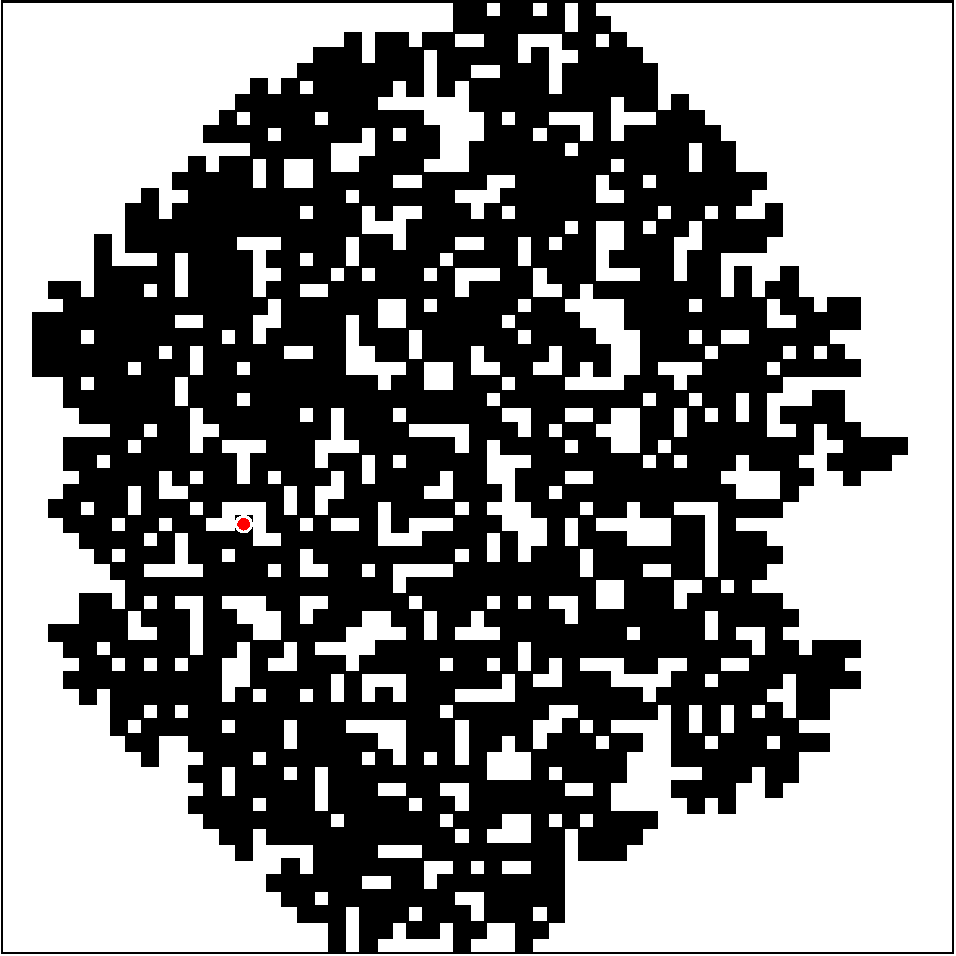
\includegraphics[width=8.0cm]{figure_1.pdf}
                        \caption{$p=0.7$としたときのパーコレーション・クラスター上をランダムウォークする蟻の例}
                        \label{fig:14-8-f1}
                    \end{center}
                \end{figure}
               
            \end{enumerate}    
        
        \item $p=0.4$のときの$\langle R^{2}(t) \rangle$を計算し,$p<p_{c}$に対してはクラスターは有限であり,$\langle R^{2}(t) \rangle$には上限があって,拡散は不可能であることを確認せよ.
            \begin{enumerate}
                \item $p=0.4$のときの$\langle R^{2}(t) \rangle$を計算し,横軸$t$,縦軸$\langle R^{2}(t) \rangle$として両対数グラフにプロットしたものを図\ref{fig:14-8-f2}に示す.グラフからも明らかなように,$p<p_{c}$ではパーコレーション・クラスターは生成されないために$\langle R^{2}(t) \rangle$には系のサイズより小さい上限(この場合7程度)があって,拡散は不可能であることがわかる.
                
                \begin{figure}[H]
                    \begin{center}
                        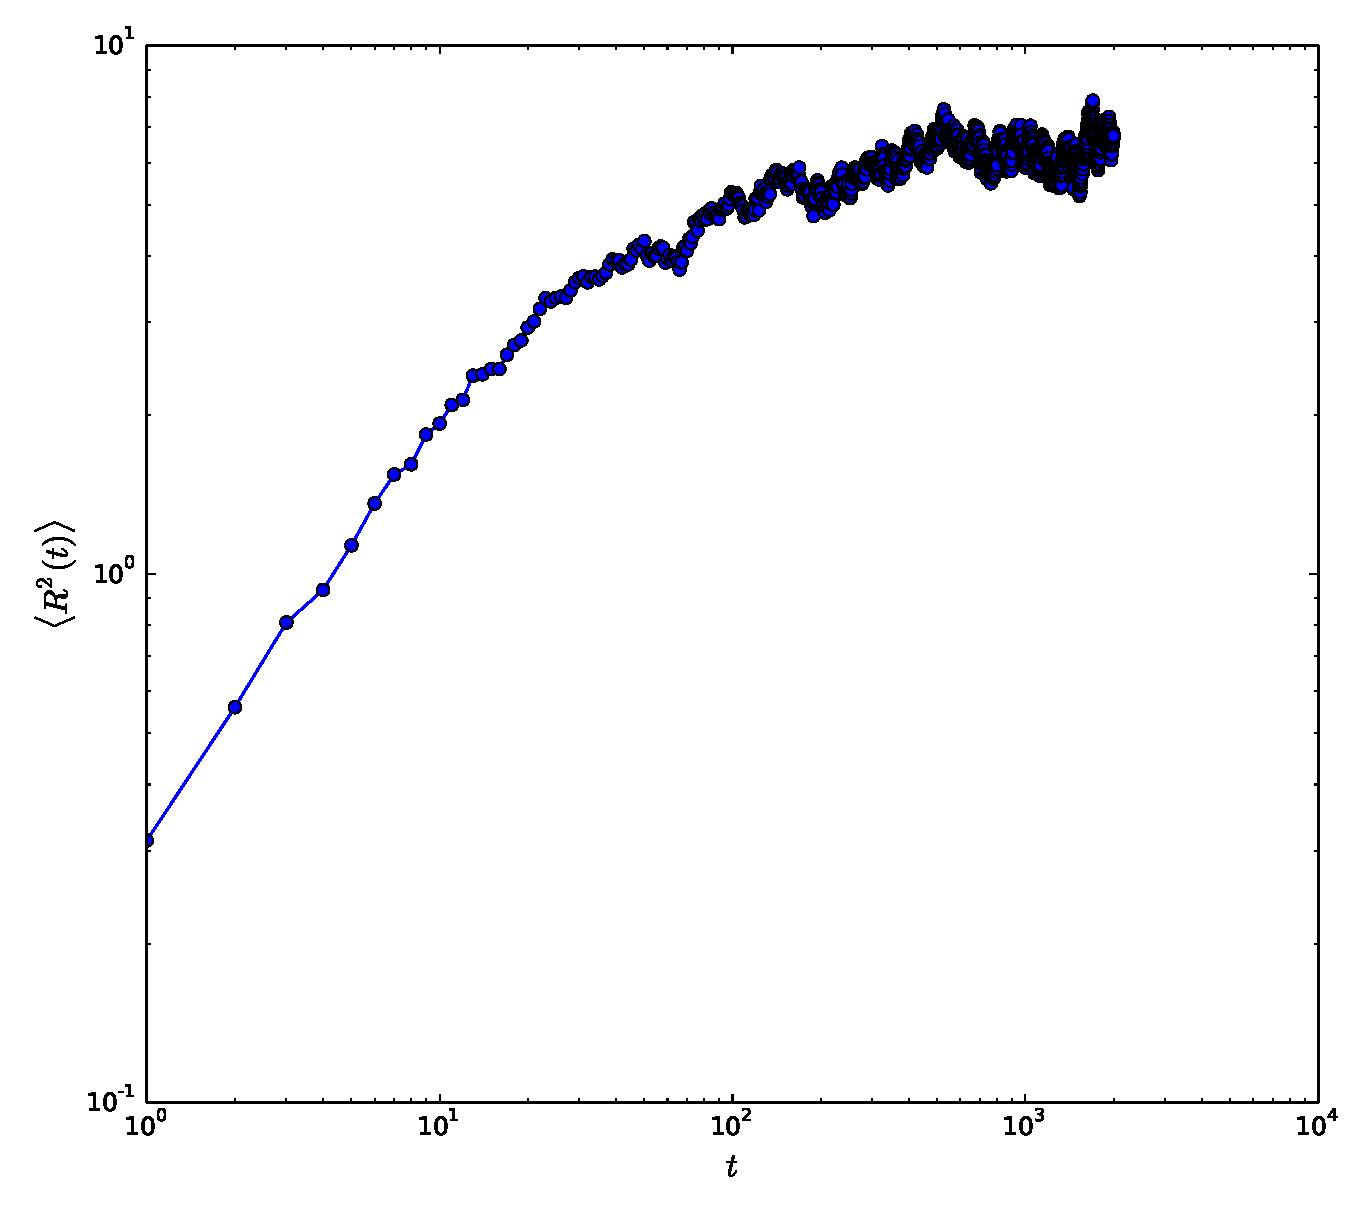
\includegraphics[width=10.0cm]{figure_2.pdf}
                        \caption{$p=0.4$のときの$\langle R^{2}(t) \rangle$.}
                        \label{fig:14-8-f2}
                    \end{center}
                \end{figure}

                
            \end{enumerate} 
        
        \item 設問aと同様に,$L=61$として$p=1.0, 0.8, 0.7, 0.65, 0.62$についての平均2乗変位を計算せよ.時間が許せば,いくつかのクラスターについての平均をとれ.$\langle R^{2}(t) \rangle$を$t$に対して両対数でプロットせよ.比較的短時間では,$\langle R^{2}(t) \rangle$の定性的な$t$依存性はどのようか.長時間について$\langle R^{2}(t) \rangle$が$t$に比例するかどうか決定せよ(格子の大きさは有限なので,$\langle R^{2}(t) \rangle$の最大値には上限があることを忘れないこと.).$\langle R^{2}(t) \rangle \sim t$の場合の$D_{s}(p)$を求めよ.比$D_{s}(p)/D(p=1)$を$p$の関数としてプロットし,定性的な振る舞いについて議論せよ.
            \begin{enumerate}
                \item $L=61$として$p=1.0, 0.8, 0.7, 0.65, 0.62$についての平均2乗変位$\langle R^{2}(t) \rangle$を計算し,両対数グラフにした(図\ref{fig:14-8-f4}).このとき,それぞれは300回の試行の平均となっている.
                
                \begin{figure}[H]
                    \begin{center}
                        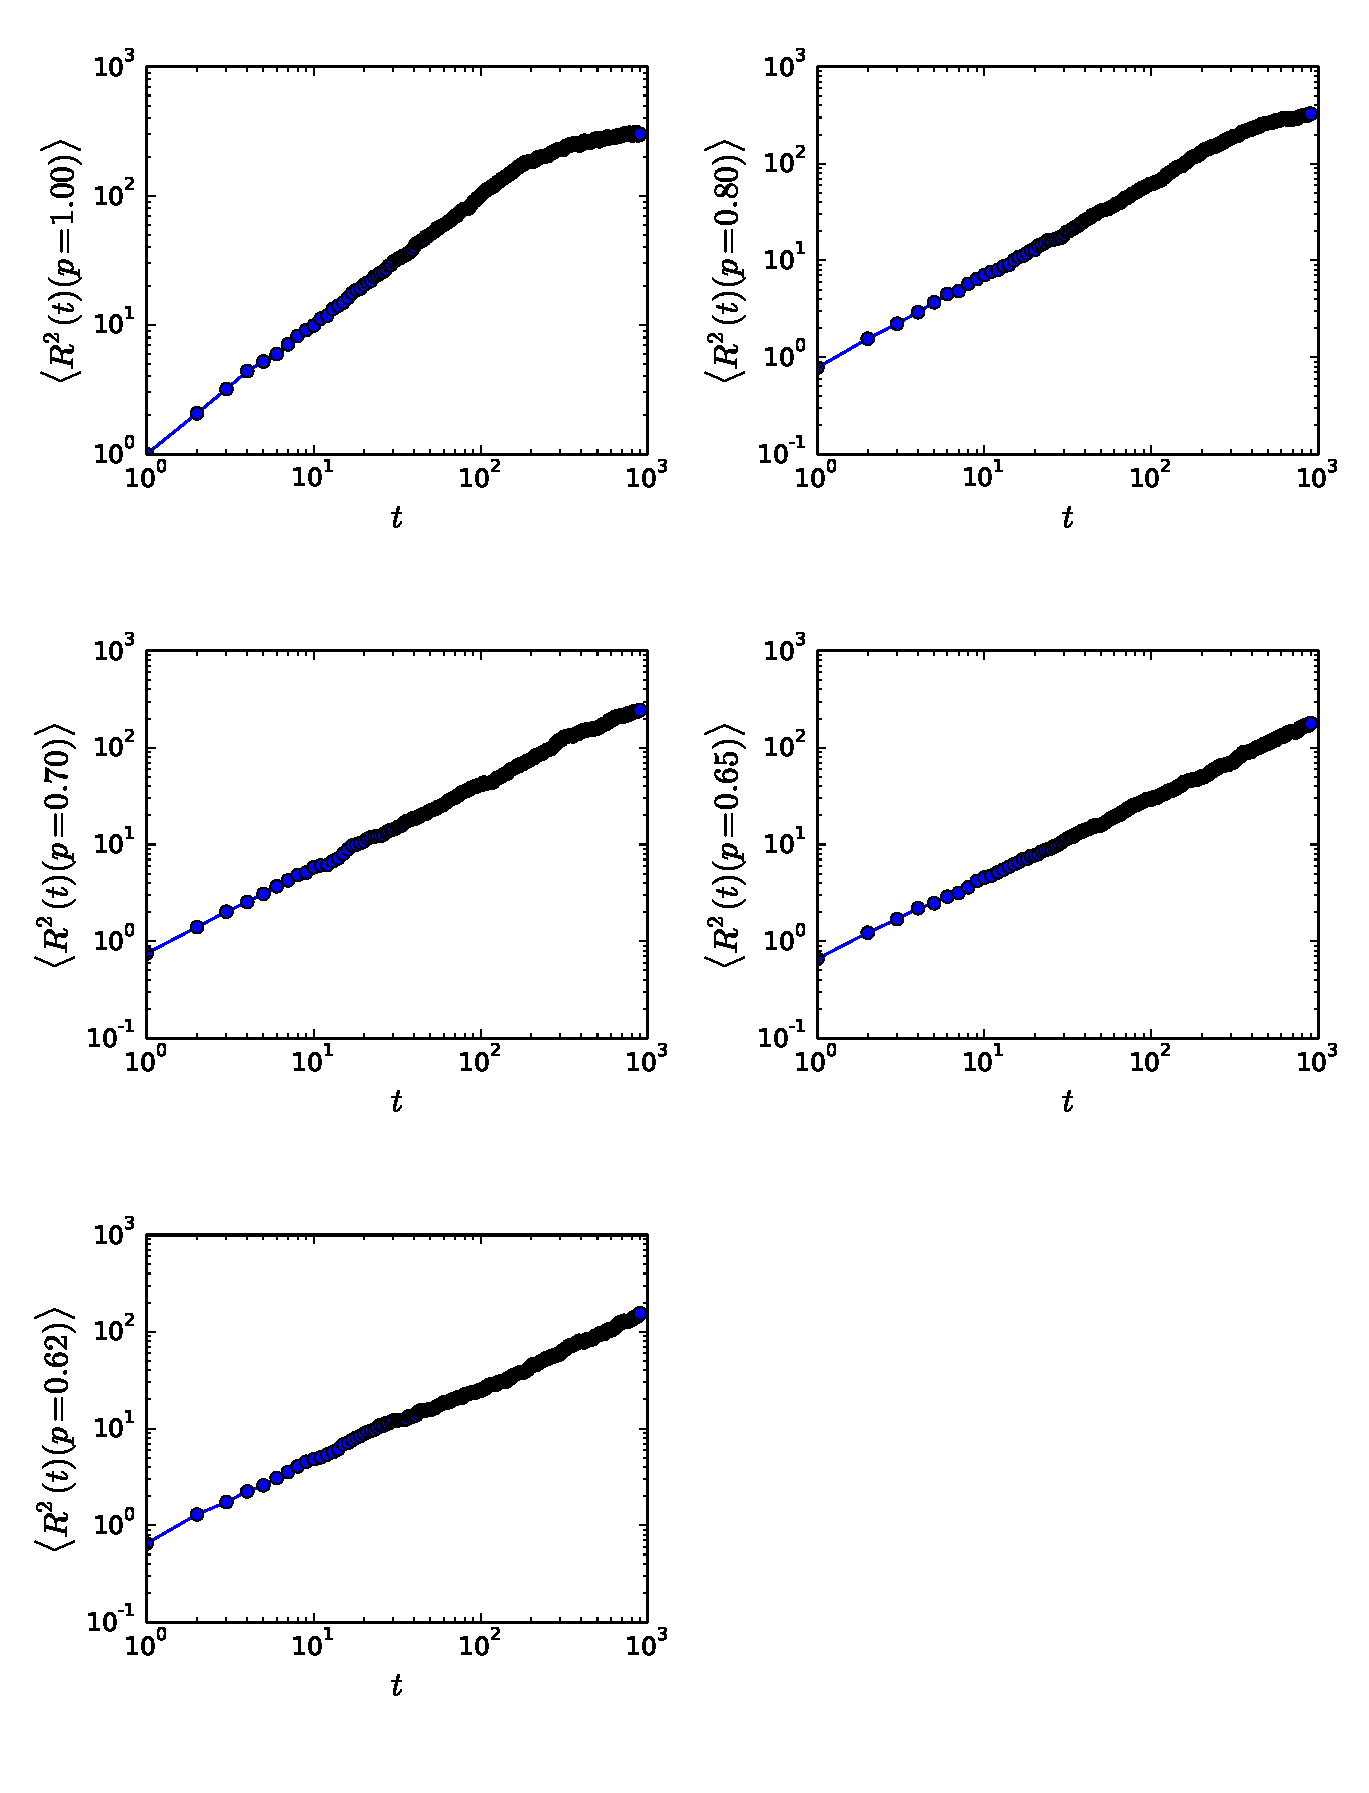
\includegraphics[width=12.5cm]{figure_4.pdf}
                        \caption{$p=1.0, 0.8, 0.7, 0.65, 0.62$についての平均2乗変位$\langle R^{2}(t) \rangle$.}
                        \label{fig:14-8-f4}
                    \end{center}
                \end{figure}

                図\ref{fig:14-8-f4}から,比較的短時間では$\langle R^{2}(t) \rangle$は$t$のべき乗で増加することがわかる.比較的長時間では,図\ref{fig:14-8-f5}に示したように,$\langle R^{2}(t) \rangle$は$t$に比例するように見える.$\langle R^{2}(t) \rangle \sim 4D_{s}(p)t$と仮定して,$D_{s}(p)$を求めると,
                $D_{s}(p=0.8)\simeq 0.0095$となった.また,同じように$p>p_{c}$の$p$に関して$D_{s}(p)$を求め,比$D_{s}(p)/D(p=1)$を$p$の関数としてプロットしたものを図\ref{fig:14-8-f6}に示す.設問dで扱われるように,$p<p_c$では拡散はないので$D_{s}$は$p\rightarrow p_{c}$とともに0になると考えられ,図\ref{fig:14-8-f6}で得られたグラフの形からも$D_{s}(p) = (p-p_{c})^{\mu_{s}}$であることが予想される.また,グラフの凸性から$\mu>1$であることもわかる.
                
                \begin{figure}[H]
                    \begin{center}
                        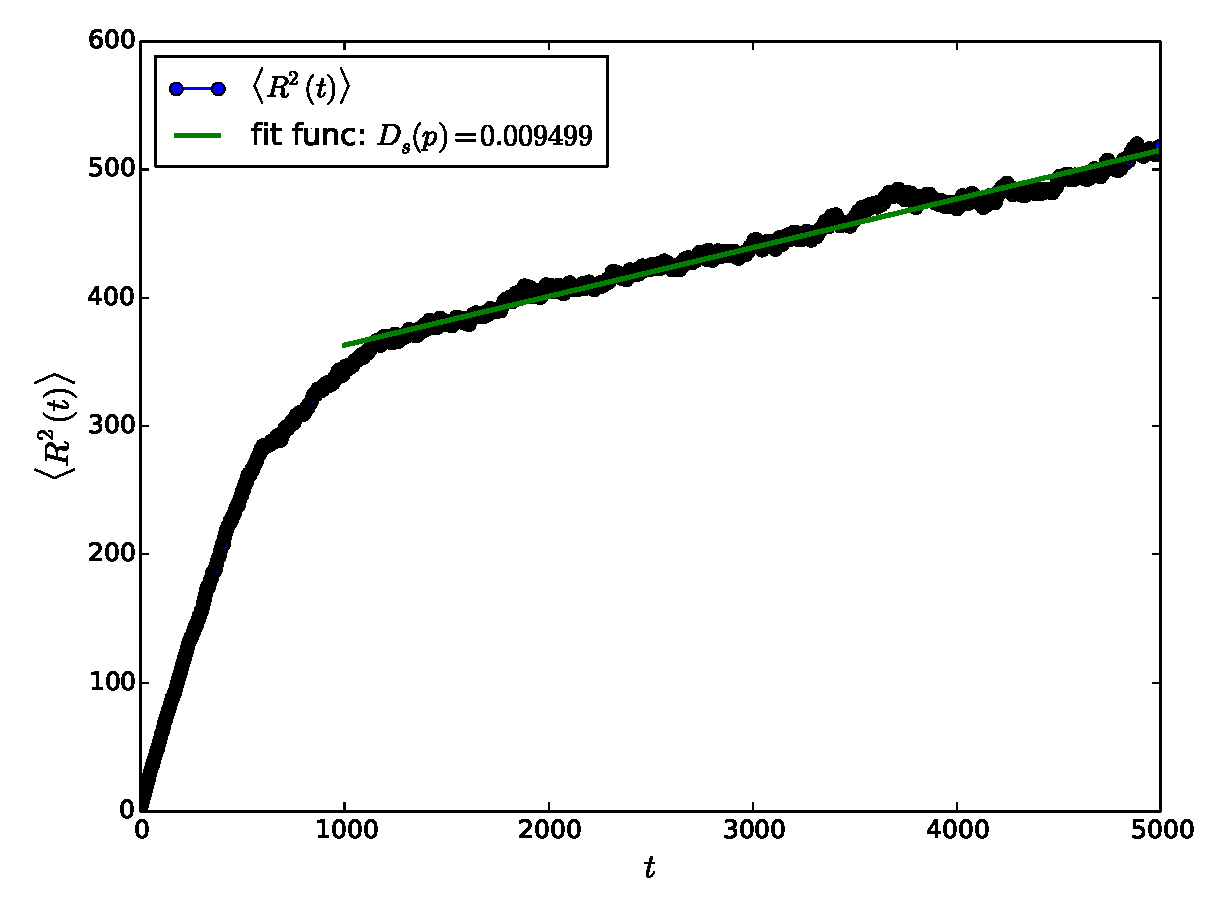
\includegraphics[width=10.0cm]{figure_6.pdf}
                        \caption{$p=0.8$で1000回の試行の平均により得られた$\langle R^{2}(t) \rangle$と$t$の関係.}
                        \label{fig:14-8-f5}
                    \end{center}
                \end{figure}
                
                \begin{figure}[H]
                    \begin{center}
                        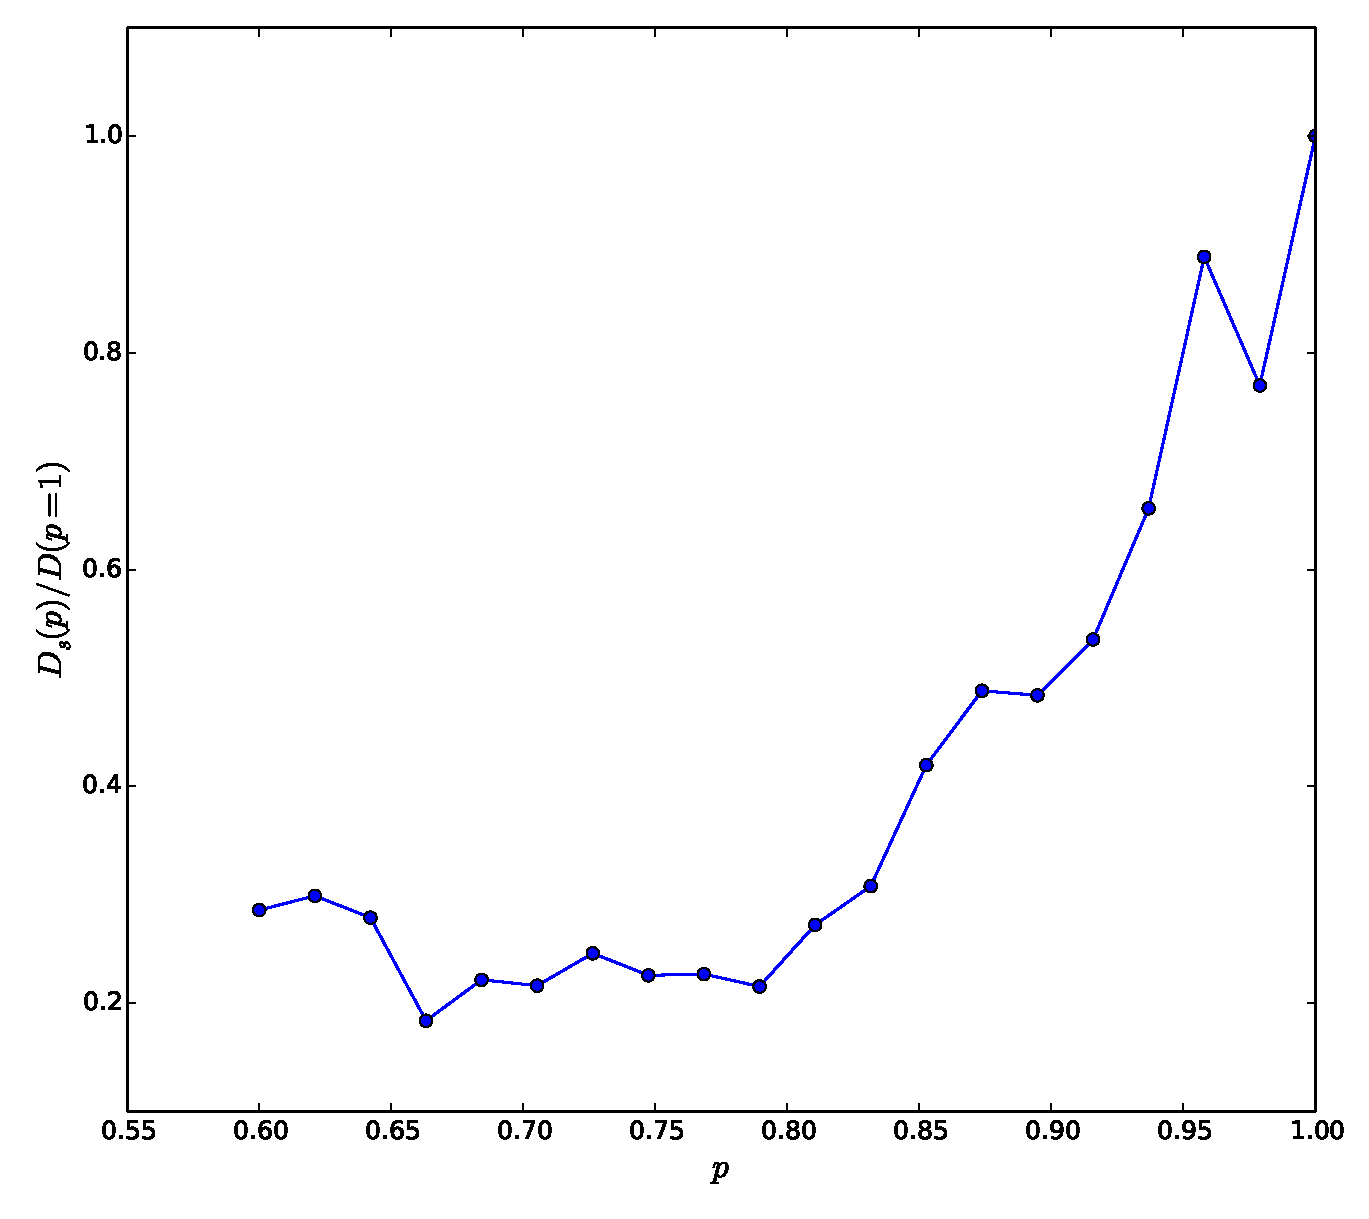
\includegraphics[width=10.0cm]{figure_7.pdf}
                        \caption{横軸$p$,縦軸を比$D_{s}(p)/D(p=1)$としてプロットしたグラフ.}
                        \label{fig:14-8-f6}
                    \end{center}
                \end{figure}

            \end{enumerate} 
        
    \end{enumerate}

\section{まとめ}
    フラクタル図形の中を拡散する粒子の運動について,その平均2乗変位$\langle R^{2}(t) \rangle$と$p$,$t$の間に成り立つ関係について,いくつかを学ぶことができた.
\nocite{textbook}
%\nocite{fractal1}
\bibliography{/home/shotaro/Workspace/computing_simulation/reference}


\end{document}
